%%%%%%%%%%%%%%%%%%%%%%%%%%%%%%%%%%%%%%%%%
% Masters/Doctoral Thesis 
% LaTeX Template
% Version 2.5 (27/8/17)
%
% This template was downloaded from:
% http://www.LaTeXTemplates.com
%
% Version 2.x major modifications by:
% Vel (vel@latextemplates.com)
%
% This template is based on a template by:
% Steve Gunn (http://users.ecs.soton.ac.uk/srg/softwaretools/document/templates/)
% Sunil Patel (http://www.sunilpatel.co.uk/thesis-template/)
%
% Template license:
% CC BY-NC-SA 3.0 (http://creativecommons.org/licenses/by-nc-sa/3.0/)
%
%%%%%%%%%%%%%%%%%%%%%%%%%%%%%%%%%%%%%%%%%

%----------------------------------------------------------------------------------------
%	PACKAGES AND OTHER DOCUMENT CONFIGURATIONS
%----------------------------------------------------------------------------------------

\documentclass[
11pt, % The default document font size, options: 10pt, 11pt, 12pt
%oneside, % Two side (alternating margins) for binding by default, uncomment to switch to one side
english, % ngerman for German
singlespacing, % Single line spacing, alternatives: onehalfspacing or doublespacing
%draft, % Uncomment to enable draft mode (no pictures, no links, overfull hboxes indicated)
%nolistspacing, % If the document is onehalfspacing or doublespacing, uncomment this to set spacing in lists to single
%liststotoc, % Uncomment to add the list of figures/tables/etc to the table of contents
%toctotoc, % Uncomment to add the main table of contents to the table of contents
%parskip, % Uncomment to add space between paragraphs
%nohyperref, % Uncomment to not load the hyperref package
headsepline, % Uncomment to get a line under the header
%chapterinoneline, % Uncomment to place the chapter title next to the number on one line
%consistentlayout, % Uncomment to change the layout of the declaration, abstract and acknowledgements pages to match the default layout
]{MastersDoctoralThesis} % The class file specifying the document structure

\usepackage[utf8]{inputenc} % Required for inputting international characters
\usepackage[T1]{fontenc} % Output font encoding for international characters

\usepackage{mathpazo} % Use the Palatino font by default

\usepackage[backend=bibtex,style=authoryear,natbib=true]{biblatex} % Use the bibtex backend with the authoryear citation style (which resembles APA)

\addbibresource{example.bib} % The filename of the bibliography

\usepackage[autostyle=true]{csquotes} % Required to generate language-dependent quotes in the bibliography

%----------------------------------------------------------------------------------------
%	MARGIN SETTINGS
%----------------------------------------------------------------------------------------

\geometry{
	paper=a4paper, % Change to letterpaper for US letter
	inner=2.5cm, % Inner margin
	outer=3.8cm, % Outer margin
	bindingoffset=.5cm, % Binding offset
	top=1.5cm, % Top margin
	bottom=1.5cm, % Bottom margin
	%showframe, % Uncomment to show how the type block is set on the page
}

%----------------------------------------------------------------------------------------
%	THESIS INFORMATION
%----------------------------------------------------------------------------------------

\thesistitle{Black-box perormance modelling and analysis of microservice systems} % Your thesis title, this is used in the title and abstract, print it elsewhere with \ttitle
\supervisor{Hui \textsc{Song}} % Your supervisor's name, this is used in the title page, print it elsewhere with \supname
\examiner{} % Your examiner's name, this is not currently used anywhere in the template, print it elsewhere with \examname
\degree{Master in Informatics} % Your degree name, this is used in the title page and abstract, print it elsewhere with \degreename
\author{Magnus \textsc{Nordbø}} % Your name, this is used in the title page and abstract, print it elsewhere with \authorname
\addresses{} % Your address, this is not currently used anywhere in the template, print it elsewhere with \addressname

\subject{Informatics} % Your subject area, this is not currently used anywhere in the template, print it elsewhere with \subjectname
\keywords{} % Keywords for your thesis, this is not currently used anywhere in the template, print it elsewhere with \keywordnames
\university{\href{http://www.university.com}{University of Oslo}} % Your university's name and URL, this is used in the title page and abstract, print it elsewhere with \univname
\department{\href{http://department.university.com}{Department Of Informatics}} % Your department's name and URL, this is used in the title page and abstract, print it elsewhere with \deptname
\group{\href{http://researchgroup.university.com}{Faculty of Mathematics and Natural Sciences}} % Your research group's name and URL, this is used in the title page, print it elsewhere with \groupname
\faculty{\href{http://faculty.university.com}{Faculty of Mathematics and Natural Sciences}} % Your faculty's name and URL, this is used in the title page and abstract, print it elsewhere with \facname

\AtBeginDocument{
\hypersetup{pdftitle=\ttitle} % Set the PDF's title to your title
\hypersetup{pdfauthor=\authorname} % Set the PDF's author to your name
\hypersetup{pdfkeywords=\keywordnames} % Set the PDF's keywords to your keywords
}

\begin{document}

\frontmatter % Use roman page numbering style (i, ii, iii, iv...) for the pre-content pages

\pagestyle{plain} % Default to the plain heading style until the thesis style is called for the body content

%----------------------------------------------------------------------------------------
%	TITLE PAGE
%----------------------------------------------------------------------------------------

\begin{titlepage}
\begin{center}

\vspace*{.06\textheight}
{\scshape\LARGE \univname\par}\vspace{1.5cm} % University name
\textsc{\Large Master's Thesis}\\[0.5cm] % Thesis type

\HRule \\[0.4cm] % Horizontal line
{\huge \bfseries \ttitle\par}\vspace{0.4cm} % Thesis title
\HRule \\[1.5cm] % Horizontal line
 
\begin{minipage}[t]{0.4\textwidth}
\begin{flushleft} \large
\emph{Author:}\\
\href{http://www.johnsmith.com}{\authorname} % Author name - remove the \href bracket to remove the link
\end{flushleft}
\end{minipage}
\begin{minipage}[t]{0.4\textwidth}
\begin{flushright} \large
\emph{Supervisor:} \\
\href{http://www.jamessmith.com}{\supname} % Supervisor name - remove the \href bracket to remove the link  
\end{flushright}
\end{minipage}\\[3cm]
 
\vfill

\large \textit{A thesis submitted in fulfillment of the requirements\\ for the degree of \degreename}\\[0.3cm] % University requirement text
\textit{in the}\\[0.4cm]
\groupname\\\deptname\\[2cm] % Research group name and department name
 
\vfill

{\large \today}\\[4cm] % Date
%\includegraphics{Logo} % University/department logo - uncomment to place it
 
\vfill
\end{center}
\end{titlepage}

%----------------------------------------------------------------------------------------
%	DECLARATION PAGE
%----------------------------------------------------------------------------------------

\begin{declaration}
\addchaptertocentry{\authorshipname} % Add the declaration to the table of contents
\noindent I, \authorname, declare that this thesis titled, \enquote{\ttitle} and the work presented in it are my own. I confirm that:

\begin{itemize} 
\item This work was done wholly or mainly while in candidature for a research degree at this University.
\item Where any part of this thesis has previously been submitted for a degree or any other qualification at this University or any other institution, this has been clearly stated.
\item Where I have consulted the published work of others, this is always clearly attributed.
\item Where I have quoted from the work of others, the source is always given. With the exception of such quotations, this thesis is entirely my own work.
\item I have acknowledged all main sources of help.
\item Where the thesis is based on work done by myself jointly with others, I have made clear exactly what was done by others and what I have contributed myself.\\
\end{itemize}

\end{declaration}

\cleardoublepage

%----------------------------------------------------------------------------------------
%	QUOTATION PAGE
%----------------------------------------------------------------------------------------

\vspace*{0.2\textheight}

\noindent\enquote{\itshape Thanks to my solid academic training, today I can write hundreds of words on virtually any topic without possessing a shred of information, which is how I got a good job in journalism.}\bigbreak

\hfill Dave Barry

%----------------------------------------------------------------------------------------
%	ABSTRACT PAGE
%----------------------------------------------------------------------------------------

\begin{abstract}
\addchaptertocentry{\abstractname} % Add the abstract to the table of contents
The Thesis Abstract is written here (and usually kept to just this page). The page is kept centered vertically so can expand into the blank space above the title too\ldots
\end{abstract}

%----------------------------------------------------------------------------------------
%	ACKNOWLEDGEMENTS
%----------------------------------------------------------------------------------------

\begin{acknowledgements}
\addchaptertocentry{\acknowledgementname} % Add the acknowledgements to the table of contents
The acknowledgments and the people to thank go here, don't forget to include your project advisor\ldots
\end{acknowledgements}

%----------------------------------------------------------------------------------------
%	LIST OF CONTENTS/FIGURES/TABLES PAGES
%----------------------------------------------------------------------------------------

\tableofcontents % Prints the main table of contents

\listoffigures % Prints the list of figures

\listoftables % Prints the list of tables

%----------------------------------------------------------------------------------------
%	ABBREVIATIONS
%----------------------------------------------------------------------------------------

\begin{abbreviations}{ll} % Include a list of abbreviations (a table of two columns)

\textbf{LAH} & \textbf{L}ist \textbf{A}bbreviations \textbf{H}ere\\
\textbf{WSF} & \textbf{W}hat (it) \textbf{S}tands \textbf{F}or\\

\end{abbreviations}

%----------------------------------------------------------------------------------------
%	PHYSICAL CONSTANTS/OTHER DEFINITIONS
%----------------------------------------------------------------------------------------

\begin{constants}{lr@{${}={}$}l} % The list of physical constants is a three column table

% The \SI{}{} command is provided by the siunitx package, see its documentation for instructions on how to use it

Speed of Light & $c_{0}$ & \SI{2.99792458e8}{\meter\per\second} (exact)\\
%Constant Name & $Symbol$ & $Constant Value$ with units\\

\end{constants}

%----------------------------------------------------------------------------------------
%	SYMBOLS
%----------------------------------------------------------------------------------------

\begin{symbols}{lll} % Include a list of Symbols (a three column table)

$a$ & distance & \si{\meter} \\
$P$ & power & \si{\watt} (\si{\joule\per\second}) \\
%Symbol & Name & Unit \\

\addlinespace % Gap to separate the Roman symbols from the Greek

$\omega$ & angular frequency & \si{\radian} \\

\end{symbols}

%----------------------------------------------------------------------------------------
%	DEDICATION
%----------------------------------------------------------------------------------------

\dedicatory{For/Dedicated to/To my\ldots} 

%----------------------------------------------------------------------------------------
%	THESIS CONTENT - CHAPTERS
%----------------------------------------------------------------------------------------

\mainmatter % Begin numeric (1,2,3...) page numbering

\pagestyle{thesis} % Return the page headers back to the "thesis" style

% Include the chapters of the thesis as separate files from the Chapters folder
% Uncomment the lines as you write the chapters

% Chapter 1

\chapter{Introduction} % Main chapter title

\label{Chapter1} % For referencing the chapter elsewhere, use \ref{Chapter1} 

%----------------------------------------------------------------------------------------

% Define some commands to keep the formatting separated from the content 
\newcommand{\keyword}[1]{\textbf{#1}}
\newcommand{\tabhead}[1]{\textbf{#1}}
\newcommand{\code}[1]{\texttt{#1}}
\newcommand{\file}[1]{\texttt{\bfseries#1}}
\newcommand{\option}[1]{\texttt{\itshape#1}}

%----------------------------------------------------------------------------------------

\section{Keywords}

Observability \\
Microservices \\
Signal-to-noise ration \\

\section{Abstract}
This thesis project aims to explore the practicality and efficacy of multivariate time series classification to quickly diagnose performance bottlenecks in a microservice system.
A simple microservice system running in Docker was forked from another project and minimally adjusted. Metrics were collected about the system using the Prometheus monitoring software, and stress testing was done at the API level with Pumba. 
The resulting data was fed into different MTS machine learning algorithms to judge their accuracy in predicting the source of the stress.
Finally, the results of these predictions were compared and the methods for collecting, treating and training on the data were documented to benefit future implementations of a similar approach.


\section{Research area and questions}
The research area for this thesis is microservices and machine learning. An inevitable intersection appears between the two fields
when the need for analysis of data from microservice systems arises. This is because these complex systems are capable of generating a 
vast amount of metric data about themselves. The amount of data is too large for a human to read, comprehend and reason about in any efficient capacity. 
This can make it very difficult to draw useful conclusions about the system. This is where machine learning comes in as a natural answer to the problem:
While humans are limited in the amount of information they can comprehend, machines typically only benefit from absurdly large datasets to draw from, as long as
the data is of acceptable quality. However, the field of machine learning applications on microservice system data is still immature as of time of writing. 
This thesis seeks to analyze a small subset of this field. The scope will be contained to identifying latency issues resulting from disproportionally high load in a part of the system, using only data from centralized logging.\\
\keyword{Research question 1}: How good are current machine learning classification algorithms at identifying causes for anomalous behavior in microservice systems?\\
\keyword{Research question 2}: What are the current main challenges to effectively utilize metric data from microservice systems?

\section{Approach}
%Researched ways of generating good data about microservice systems to use
%Used microservices-demo and its limited collection
%Purpose became to find what one could from the limited data that was collected.
To research these questions and try to create meaningful results that can have a real impact, I formulated a hypothesis to work as the base for the project. 
\textbf{\textit{It is possible to use stress testing software and centralized logging to create a machine learning model of the system behavior to classify and identify sources of latency in a microservice system.}}
To test this hypothesis, a fork of the open source demo microservice project "sockshop" by Weaveworks was used \cite*{Microservices-demo-sockshop}. This system was hosted on a local machine and stress tested using various configurations.
Locust, an API stress testing tool. The full spectrum of available Prometheus metric data was collected in 601 time series features into csv files and labeled. There were a total of five classes, representing different endpoints connecting to different underlying microservices.
This data was then analyzed both manually and mathematically, and preprocessed to reduce noise and extract important features. 
Several methods of preprocessing and classifying were quantitatively compared. Finally, the results of the analysis were discussed and conclusions drawn.

\section{List of important terms}
\begin{itemize}
\item \keyword{Dynamic Time Warping}: A method of statistically comparing time series across time points to judge similarity.
\item \keyword{Multivariate Time Series (MTS)}: Time series data with two or more variables.
\item \keyword{Instance}: All the data collected from a system in a specific time frame, represented as an MTS.
\item \keyword{Feature}: A unique variable in the time series that expresses some kind of information about the system. Collected at fixed intervals to form an MTS.
\item \keyword{Time frame}: The period of time recorded in a time series. Each instance in this thesis corresponds to a specific time frame.
\item \keyword{Centralized logging}: Umbrella term for various microservice info logging methods that collect logs from individual microservices and stores them together. 
\item \keyword{Distributed tracing}: 
\end{itemize}

\keyword{Appendices} -- this is the folder where you put the appendices. Each appendix should go into its own separate \file{.tex} file. An example and template are included in the directory.

\keyword{Chapters} -- this is the folder where you put the thesis chapters. A thesis usually has about six chapters, though there is no hard rule on this. Each chapter should go in its own separate \file{.tex} file and they can be split as:
\begin{itemize}
\item Chapter 1: Introduction to the thesis topic
\item Chapter 2: Background information and theory
\item Chapter 3: (Laboratory) experimental setup
\item Chapter 4: Details of experiment 1
\item Chapter 5: Details of experiment 2
\item Chapter 6: Discussion of the experimental results
\item Chapter 7: Conclusion and future directions
\end{itemize}
This chapter layout is specialised for the experimental sciences, your discipline may be different.

\keyword{Figures} -- this folder contains all figures for the thesis. These are the final images that will go into the thesis document.


\section{Thesis Features and Conventions}\label{ThesisConventions}

To get the best out of this template, there are a few conventions that you may want to follow.

One of the most important (and most difficult) things to keep track of in such a long document as a thesis is consistency. Using certain conventions and ways of doing things (such as using a Todo list) makes the job easier. Of course, all of these are optional and you can adopt your own method.

\subsection{Printing Format}

This thesis template is designed for double sided printing (i.e. content on the front and back of pages) as most theses are printed and bound this way. Switching to one sided printing is as simple as uncommenting the \option{oneside} option of the \code{documentclass} command at the top of the \file{main.tex} file. You may then wish to adjust the margins to suit specifications from your institution.

The headers for the pages contain the page number on the outer side (so it is easy to flick through to the page you want) and the chapter name on the inner side.

The text is set to 11 point by default with single line spacing, again, you can tune the text size and spacing should you want or need to using the options at the very start of \file{main.tex}. The spacing can be changed similarly by replacing the \option{singlespacing} with \option{onehalfspacing} or \option{doublespacing}.

\subsection{Tables}

Tables are an important way of displaying your results, below is an example table which was generated with this code:

{\small
\begin{verbatim}
\begin{table}
\caption{The effects of treatments X and Y on the four groups studied.}
\label{tab:treatments}
\centering
\begin{tabular}{l l l}
\toprule
\tabhead{Groups} & \tabhead{Treatment X} & \tabhead{Treatment Y} \\
\midrule
1 & 0.2 & 0.8\\
2 & 0.17 & 0.7\\
3 & 0.24 & 0.75\\
4 & 0.68 & 0.3\\
\bottomrule\\
\end{tabular}
\end{table}
\end{verbatim}
}

\begin{table}
\caption{The effects of treatments X and Y on the four groups studied.}
\label{tab:treatments}
\centering
\begin{tabular}{l l l}
\toprule
\tabhead{Groups} & \tabhead{Treatment X} & \tabhead{Treatment Y} \\
\midrule
1 & 0.2 & 0.8\\
2 & 0.17 & 0.7\\
3 & 0.24 & 0.75\\
4 & 0.68 & 0.3\\
\bottomrule\\
\end{tabular}
\end{table}

You can reference tables with \verb|\ref{<label>}| where the label is defined within the table environment. See \file{Chapter1.tex} for an example of the label and citation (e.g. Table~\ref{tab:treatments}).

\subsection{Figures}

There will hopefully be many figures in your thesis (that should be placed in the \emph{Figures} folder). The way to insert figures into your thesis is to use a code template like this:
\begin{verbatim}
\begin{figure}
\centering

\includegraphics{Figures/Electron}
\decoRule
\caption[An Electron]{An electron (artist's impression).}
\label{fig:Electron}
\end{figure}
\end{verbatim}
Also look in the source file. Putting this code into the source file produces the picture of the electron that you can see in the figure below.

\begin{figure}[th]
\centering

\includegraphics{Figures/Electron}
\decoRule
\caption[An Electron]{An electron (artist's impression).}
\label{fig:Electron}
\end{figure}

Sometimes figures don't always appear where you write them in the source. The placement depends on how much space there is on the page for the figure. Sometimes there is not enough room to fit a figure directly where it should go (in relation to the text) and so \LaTeX{} puts it at the top of the next page. Positioning figures is the job of \LaTeX{} and so you should only worry about making them look good!

Figures usually should have captions just in case you need to refer to them (such as in Figure~\ref{fig:Electron}). The \verb|\caption| command contains two parts, the first part, inside the square brackets is the title that will appear in the \emph{List of Figures}, and so should be short. The second part in the curly brackets should contain the longer and more descriptive caption text.

The \verb|\decoRule| command is optional and simply puts an aesthetic horizontal line below the image. If you do this for one image, do it for all of them.

\LaTeX{} is capable of using images in pdf, jpg and png format.

\subsection{Typesetting mathematics}

If your thesis is going to contain heavy mathematical content, be sure that \LaTeX{} will make it look beautiful, even though it won't be able to solve the equations for you.

The \enquote{Not So Short Introduction to \LaTeX} (available on \href{http://www.ctan.org/tex-archive/info/lshort/english/lshort.pdf}{CTAN}) should tell you everything you need to know for most cases of typesetting mathematics. If you need more information, a much more thorough mathematical guide is available from the AMS called, \enquote{A Short Math Guide to \LaTeX} and can be downloaded from:
\url{ftp://ftp.ams.org/pub/tex/doc/amsmath/short-math-guide.pdf}

There are many different \LaTeX{} symbols to remember, luckily you can find the most common symbols in \href{http://ctan.org/pkg/comprehensive}{The Comprehensive \LaTeX~Symbol List}.

You can write an equation, which is automatically given an equation number by \LaTeX{} like this:
\begin{verbatim}
\begin{equation}
E = mc^{2}
\label{eqn:Einstein}
\end{equation}
\end{verbatim}

This will produce Einstein's famous energy-matter equivalence equation:
\begin{equation}
E = mc^{2}
\label{eqn:Einstein}
\end{equation}

All equations you write (which are not in the middle of paragraph text) are automatically given equation numbers by \LaTeX{}. If you don't want a particular equation numbered, use the unnumbered form:
\begin{verbatim}
\[ a^{2}=4 \]
\end{verbatim}

%----------------------------------------------------------------------------------------

\section{Sectioning and Subsectioning}

You should break your thesis up into nice, bite-sized sections and subsections. \LaTeX{} automatically builds a table of Contents by looking at all the \verb|\chapter{}|, \verb|\section{}|  and \verb|\subsection{}| commands you write in the source.

The Table of Contents should only list the sections to three (3) levels. A \verb|chapter{}| is level zero (0). A \verb|\section{}| is level one (1) and so a \verb|\subsection{}| is level two (2). In your thesis it is likely that you will even use a \verb|subsubsection{}|, which is level three (3). The depth to which the Table of Contents is formatted is set within \file{MastersDoctoralThesis.cls}. If you need this changed, you can do it in \file{main.tex}.

%----------------------------------------------------------------------------------------

\section{In Closing}

You have reached the end of this mini-guide. You can now rename or overwrite this pdf file and begin writing your own \file{Chapter1.tex} and the rest of your thesis. The easy work of setting up the structure and framework has been taken care of for you. It's now your job to fill it out!

Good luck and have lots of fun!

\begin{flushright}
Guide written by ---\\
Sunil Patel: \href{http://www.sunilpatel.co.uk}{www.sunilpatel.co.uk}\\
Vel: \href{http://www.LaTeXTemplates.com}{LaTeXTemplates.com}
\end{flushright}

%\chapter{Background}

\label{Chapter2}

This section will present the main concepts that are relevant to the thesis project and the reason why it's useful.
It will first explain the main theory behind microservices and how it seeks to solve the main problems in legacy software architectures. Then it will
detail the new issues that arise from microservices. Finally, it will paint a picture of today's landscape of distributed software and 
tie it all together to explain the value of the research in this project.

\section{The monolith}
In general when talking about both microservices and distributed computing in general, the concept of a \textbf{Monolith} often gets brought up. 
The monolith is this concept of a large, self-contained application where all the code and functionality is tightly bundled together, and is very hard to separate into individual parts.
The definition has changed over time: According to the ITS back in 2001 \cite{ITS}, a monolith was "An application in which the user interface, business rules, and data access code is combined into a single executable program and deployed on one platform."
However, most modern interpretations online refer back to a book from 2003 called \textit{The art of Unix programming}. Usually referred to as "monster monoliths", it marks the beginning of the trend of using the term monolith as a bogeyman of unmaintainable, poorly planned code. 
This trend has been continued in modern days with software "gurus" and the like when needing something to compare to our lord and savior microservices \cite*{Gouigoux2017}.
It is therefore important to remember that:
\begin{enumerate}
    \item The monolith is not a defined software architecture design paradigm. Rather, it is the default type of application that appears when not taking great effort and intentionality to split the code up in many distinct parts.
    \item The monolith is not some damnable evil to be conquered: On software projects of a less-than-huge scale, it is very often quite optimal. It doesn't have to deal with inter-component communication. Keeping everything contained in one code base makes it easy to run and test on local machines, keeps all the code in one place for easy access, and so on. 
    \item The monolith mostly just exists as a concept when talking about microservices or other ways to break it up. Its purpose is mainly to demonstrate the benefits of code splitting in large software.
\end{enumerate}

With that out of the way, let's discuss the problems with monolithic software that microservices seek to amend.\\
The core issue that with monolithic software is \textbf{entanglement.}
In this context, it means how complex monolithic software will have too many interconnected, interdependent parts to manage effectively.
This interdependence will mean that something that is a problem for one small part of the whole, will be a problem for the entire tech stack. 

\subsection{Scalability} 
Scalability refers to the ability to increase the workload capacity of the software \cite*{Scalability}. 
If the amount of users, data, geographical reach or computation complexity increases, it becomes necessary to increase hardware capabilities. 
Scaling up monolithic software can be a time-consuming and costly affair, as it usually doesn't allow for only increasing the capacity of the parts of the software that are facing increased load.  \\
An example: 
\begin{quote} 
 On the 24th of December 2004, Delta Air Lines' crew scheduling system crashed because of an integer overflow bug resulting from record system load. 
 It took 24 hours of frantic work to implement a workaround that duplicated a database \cite*{USAToday}. 
It used an old flight scheduling system called TRACK from 1986 to organize scheduling. 
Their database that handled pilots and flight attendants ran into a hard limit at 32000 entries.
The hotfix for this problem was to spin up another server, and let one database only handle pilots and another only handle flight attendants. 
The crash caused widespread disruptions. According to the Department of Transportation of the US, approximately 269,000 passengers were affected by delays and cancellations \cite*{DOT}. 
\end{quote}
Issues from heavy loads like this are always a risk. But entangled monolith systems are not easy to extend. 
In a microservices oriented system, implementing this extension fix would likely be on the scale of modifying a few lines of code and spinning up another instance of the database. 
I highlight this example because the fix for this huge problem ended up being a basic principle of microservices: Generating more instances of only the overloaded components. 
\\
When an application has reached load capacity, one realistically has two options \cite*{Scalability}:
\begin{enumerate}
    \item Improve the efficiency of the software, so it can serve higher loads with the same hardware
    \item Upgrade the hardware
\end{enumerate}
Naturally, the software improvement solution will only get you so far. It has the added issue of (in this example) being a monolithic application, so big changes to the software is a time consuming and costly project.\\
When upgrading the hardware capacity of monolithic applications, it often becomes a project of its own. One with expenses. 
Because of this, and the fact that monolithic application will have to be replicated in its entirety on the new server by default, a scaling project will try to calculate the future growth of the user base and invest in a solution that will be able to handle user load for the foreseeable future.
This is a point of potential failure, as being wrong about future growth could turn out to be quite costly.
\begin{figure}[ht] 
\centering 
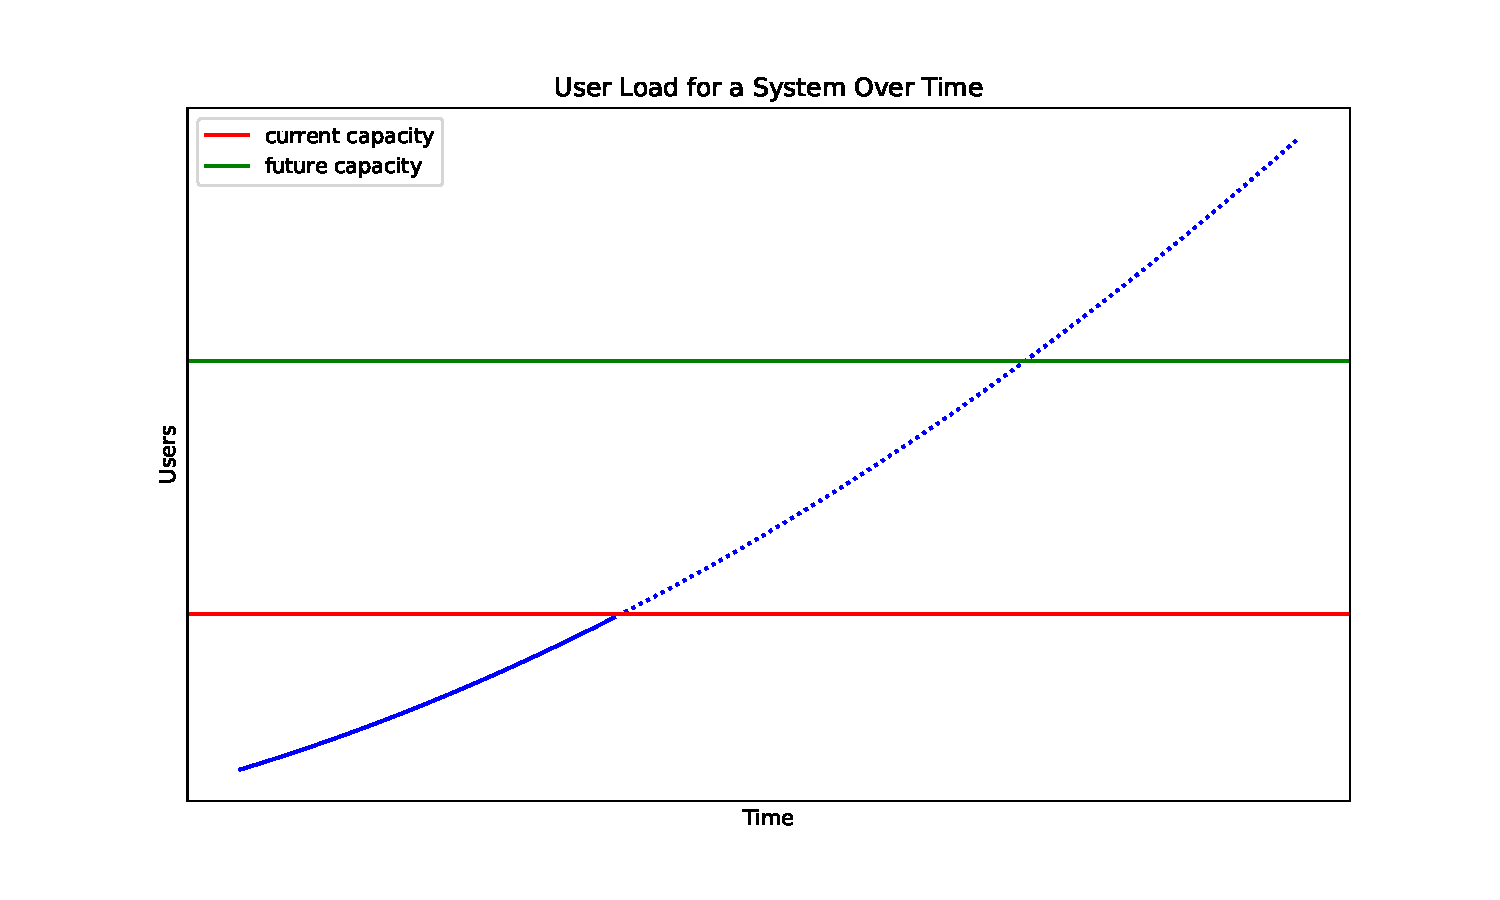
\includegraphics[width=0.8\columnwidth]{Figures/Graphs/capacity_scaling.pdf}
\caption{Scaling a monolith requires making assumptions about future growth}
\label{Monolith scaling}
\end{figure}

\subsection{Comprehension}
Comprehension of large software is impossible. 
There is a human limit to how much one can keep in one's mind. 
In large software, the amount of functions and interactions can balloon into the tens or hundreds of thousands. 
Fully comprehending such a system is impossible for human brains, and it becomes necessary to abstract it down to a manageable mental model. 
Without good comprehension of the system, it is very difficult to make good changes, adjustments or additions.
A highly entangled monolith can very difficult to abstract, without clear boundaries for which parts do what.

\subsection{Modern software development}
Modern software development is characterized by autonomous teams working separately and collaborating through continuous integration. 
This means: build often, test often, merge often. 
According to Agile practices, one should write tests first, then write code that passes the tests. 
But writing tests for highly entangled monolithic software is challenging, as even small changes can have consequences far down the chain. 
Building often will also become costly: Monolithic software will typically need to be rebuilt from scratch each time. 
A costly affair, and entirely unfeasible if the goal is to build several times a day. 

\subsection{Resilience}
Resilience has several definitions in the context of software. \cite*{Curtis}. 
In the context of this thesis, we can define it as "the ability to keep running correctly in spite of failures". Often called fault tolerance.
The entanglement of the monolith once again becomes a problem here. 
A single function running into an unexpected situation and throwing an error will, by default in most technologies, abort the execution of the program entirely.
It can be circumvented by try/catch statements and other error handling methods, but an entangled system is extremely difficult to make fault tolerant.

\subsection{Technical debt} 
Technical debt is a somewhat loosely defined term. It is defined by Steve McConnell as \textit{A
design or construction approach that's expedient in the short term, but
that creates a technical context in which the same work will cost more
to do later than it would cost to do now (including increased cost over
time) \cite*{McConnell2013}.”}
As a monolithic application grows, making any change becomes a larger project.
The more entangled everything is, the more changes will have to be made to accommodate updated dependencies or changes in behavior. 
These changes to accommodate the change can also cause other things to be changed.
This is often called the "ripple effect" or "cascading changes". 
This can lead to mounting technical debt: As updating components is such a project, it is delayed, or jury rigged to work in the short term.
But each delay or subpar implementation leads to an increase in how big of a project it would be to properly update dependencies.
Technical debt will also make regular maintenance more difficult and time consuming over time. 
Technical debt is not a problem that is unique to monoliths. 
But it is hard to pay off that debt through refactoring and maintenance in an entangled system that handles change poorly.

\section{Containers}
Containers are a technology that packages a unit of software and all its required dependencies.
They make use of the Linux kernel's namespaces feature.
Namespaces partition system resources in a way that processes only "see" the resources in their namespace, instead of the total system resources. 
This provides a level of abstraction and security, as processes can only access their own namespace.
By utilizing namespaces, containers can provide isolated workspaces for processes, essentially allowing applications to run in their own "virtual" system, oblivious to other processes running on the same host.
This makes containers completely dependency and OS agnostic,
since each container comes with the OS and packages they need to run their process.
Containers are similar to virtual machines, but much faster and more lightweight.
VMs virtualize the hardware and entire OS, like RAM and the kernel, and then run their OS on the virtualized hardware. 
Containers simply virtualize the OS, running it on their assigned namespace on the host's kernel.
This takes far fewer system resources at a slight cost to isolation.
This makes them viable as a way to organize code segments.
Containers talk to each other using regular network calls. 
Because of this, an application can freely be split up between several machines.

\begin{figure}[ht] 
\centering 
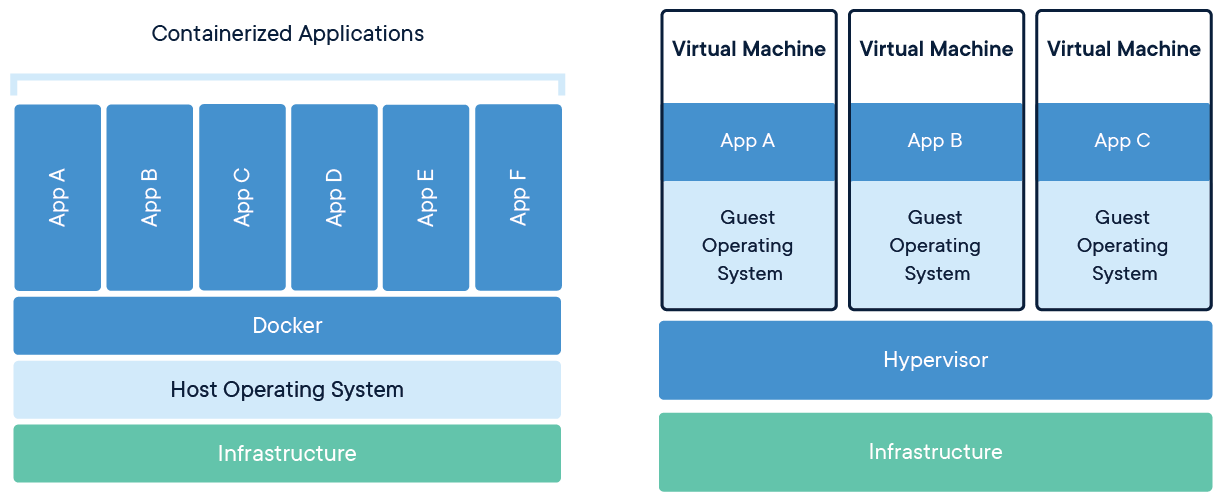
\includegraphics[width=\columnwidth]{Figures/containers_vs_VMs.png}
\caption{Containers vs VMs. Image credit: Docker inc}
\label{Containers}
\end{figure}


\section{The microservice}
The core idea of microservices is modularization, which has been a concept in software engineering since its inception. 
Microservices are a modern spin on the concept with cloud and DevOps in mind. 
The defining feature of the microservice is the container. 
By splitting the code of a piece of software into several autonomous containers that talk to each other using web requests, 
one can counter a majority of the problems with large software projects. \\
Let's examine how microservices tackle the main problems with monolithic software.

\subsection{Scalability}
Microservices are designed to be very easy to scale. 
Because the containers in a microservice system talk to each other using network calls anyway, a microservice system does not particularly care \textit{where} the containers are located.
This means you can gracefully distribute the software across servers and spin up only however many instances of each microservice you need.
This works well with modern server renting solutions, that let you pay for only what you need. 
In this way, the aforementioned scaling project for monoliths that try to calculate future growth becomes unnecessary. 
One can simply scale out only what one needs, when one needs.

\begin{figure}[ht] 
    \centering 
    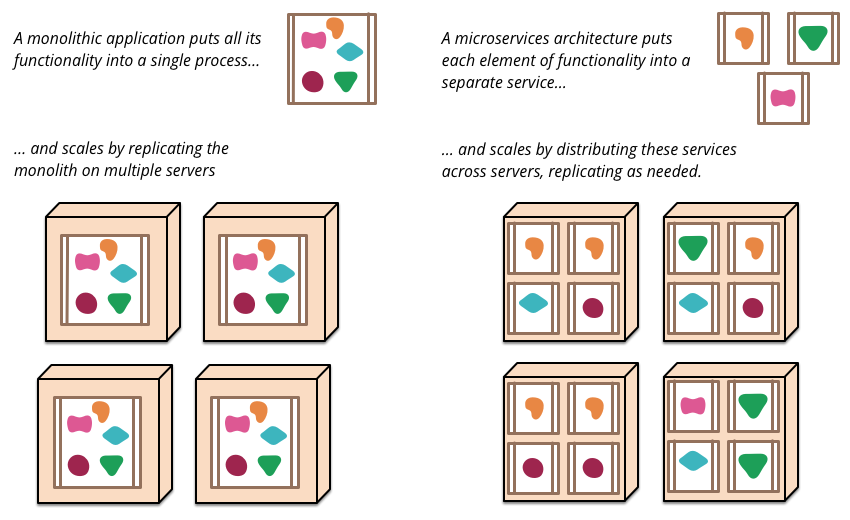
\includegraphics[width=\columnwidth]{Figures/scaling.png}
    \caption{Illustrating how monoliths and microservices handle scaling. Credit: Martin Fowler \cite*{Fowler2014}}
    \label{Scaling-comparison}
\end{figure}

\subsection{Comprehension}
Microservices promise to make complex software easier to work with. 
It does not typically do this by reducing complexity, but by providing real, traceable boundaries between units of software, and by use of interfaces.
By software boundaries, I mean that developers have an objective rule to follow for breaking code up into pieces that can be mapped out and abstracted.
Without microservices one can still map out a program, but the boundary lines between units can often be hard to nail down in a satisfying manner.
Functions are a natural "unit" to break a program up into, but functions vary a lot in size, scope, and utility.
Mapping out a program or its states, for example in UML, requires reasoning about a level of abstraction to use in the current map context. 
This decided level of abstraction will likely need to represent some functions by themselves, while grouping others together. 
While this is not necessarily a bad thing, it makes the process of mapping out a program require skilled, subjective reasoning. 
Microservices, on the other hand, provide an objective boundary that makes sense in the context of mapping out a program to comprehend it.
Thus, as long as the microservice architecture itself is well thought out (which is not guaranteed at all), no skill is necessary to create a logical abstraction of the system that is guaranteed to be useful for comprehension.\\

Interfaces are the intended inputs and outputs of each microservice. 
They help comprehension by letting developers think of the rest of the program as a black box, and only focus on comprehending the parts of the program that interact with the microservice they are currently working on.
They don't have to know what the entirety of the system does to make good changes (in theory).

\subsection{Modern software development}
The modern day is a time of DevOps and agile development.
The core principles of DevOps is up for some debate \cite*{Devops-definition}, but can be roughly summarized to be a set of guiding principles to facilitate communication and collaboration between developers and operators (hence the name DevOps). 
It places emphasis on continuous integration, delivery, and deployment (CI/CD). 
Microservices are often regarded as a core component of DevOps \cite*{Devops-amazon}.
The independence of microservices aligns well with DevOps principles. 
Each service can be developed, tested, deployed, and monitored independently, allowing for more frequent updates and releases. 
This plays into the CI/CD model central to DevOps: updates are continually integrated into the software, tested, and then deployed. 
By breaking down the application into smaller services, teams can manage and maintain their CI/CD pipelines more effectively, each focusing on their own service.\\
\\
Microservices also fit well within Agile methodologies. 
Agile focuses on iterative development, where software is developed in small pieces, with stakeholder feedback incorporated along the way. 
Microservices support this iterative approach by allowing teams to work on different services simultaneously.
\subsection{Resilience}
The ability to handle faults, crashes and unexpected occurrences is crucial to modern software platforms that provide necessary services to large parts of the population. 
Modern microservice technologies and services, like Kubernetes, OpenShift, Rancher, Google Kubernetes Engine (GKE), Azure Kubernetes Service (AKS), and many more, provide automatic load balancing and self healing. 
This means that they will detect faults and spin up new instances of the microservices to take over the workload of the failing service. 
This makes microservice applications much more robust than monoliths, which are constantly at great danger of letting a single fault bring the whole service down.

\subsection{Technical debt}
The way microservices help deal with technical debt is by making it easier in general for developers to make changes and adjustments to the system.
That is to say, technical debt will accumulate in microservice architecture just like it does in monoliths. 
It is just that the more robust and changeable microservice system is easier to refactor individual parts of the system.
This is achieved through the total separation of components that talk to each other through \textbf{interfaces}. 
The interface in this context just means the expected inputs and outputs of each microservice.
Each individual microservice is "blind" to what goes on in the others, and treat them as black boxes.
All they care about is the interface: If what goes into a service and what comes out of it has the same properties as before, a microservice system will not notice a change even if the entire technology stack of the microservice is replaced.
This makes updating to new technology a much simpler process: A developer just has to make sure it can receive and send the same data as before, and not worry any further about ripple effects.

\section{The problems with microservices}
Microservices solve many problems with legacy software, but it also introduces issues of its own. 
The problems that microservices create have largely to do with complexity.
The reality is that microservices aren't less complex than monoliths, they just exchange one type of complexity for another. 
One that, it is argued, is easier to deal with. It leads to issues nonetheless.
This section will give a detailed overview of the problems that microservices introduces.

\subsection{Complexity}
Microservices do not reduce complexity: They simply exchange one type of complexity for another. 
The issues with complexity in microservices come from the architecture itself, and from the fact that it is so loosely coupled that it allows for any technology stack and programming language.\\
Microservice has to orchestrate and manage many, many nodes. 
The scaling method of creating more instances of microservices that are struggling to handle load is great for easy scaling, but it can easily become a nightmare to manage.
When multiple instances of the same service are to cooperate, care has to be taken to split the workload in a good manner.
Careless management can lead to race conditions, data getting lost, or tasks being done several times in a redundant fashion.\\
Larger systems will have hundreds or thousands of microservices that need to communicate with each other in a complex web that is difficult or impossible to comprehend.
Orchestrating and managing this complex web of web requests is a field still in development.

\subsection{Communication overhead}
The decoupled nature of microservices comes at a concrete cost in communication overhead.
If one compares two equally well made services of equal function and size, one running on a monolith and one on microservices, the monolith should have less latency and better performance.
The cost of communication is twofold: Complexity (as mentioned above), and resource usage.
There are ways to organize connection complexity, like event-driven architecture (EDA), service mesh solutions (Istio, Linkerd, Cosnul) or serverless architecture solutions like AWS Lambda, which abstract the network away from the developer entirely.
But all of these solutions need computing power and bandwidth to work, which means they come at a cost of performance. \\
There is also the issue of the various units of code communicating with each other through network requests.
This is, in many ways, the secret sauce that makes microservices so reliable and scalable. 
But function calls are faster and less resource intensive than network requests by an order of magnitude. 
Internal function calls just deals with local memory, and their speed is measured in nanoseconds.
Meanwhile, network requests are typically measured in milliseconds. 
The distributed nature of the microservices also mean that a service could be needing to communicate with another server on a different place on the planet.
This is also a significant factor for latency, and can be a bottleneck for service quality.


\subsection{Data consistency}
Data consistency (and the lack thereof) is another complexity trade-off in microservices architecture.
While implementations vary, it is common for microservices to each have their own little database for storing data relevant to their work.
This leads to resilience, but also means that changed values may take time to propagate to all relevant microservices, leading to microservices potentially disagreeing on the value of certain variables.
This can lead to inconsistent data, where an end user might get a different result depending on time of day or where they are pinging the service from.\\
Updating data can be a challenging affair. If, for example, there is a network of 100 microservices that need to be updated with new data, that is 100 potential points of failure.
If data consistency is important, changes would need to be rolled back if any of the 100 transactions fail. 
That would require noticing a fault occurred, then notifying all the services that changed successfully that they must roll back, introducing more potential points of failure.
The most common implementation of this is the \textit{two-phase commit protocol} (2PC). 
It works by assigning one node as the coordinator/master, who sends a query to commit message to all other nodes.
All nodes then vote, by performing some internal check to see if it could successfully commit the proposed change.
If all nodes voted yes, then a commit message is sent from the coordinator/master to perform the change.
This process does a pretty good job at ensuring data consistency, but has many potential issues.
While the core algorithm itself is pretty simple, the actual implementation ends up being complex because it has to include protocols for many types of issues \cite*{Samaras2009}.    

\subsection{Testing and debugging}
 
%\chapter{Data processing}

\section{Imputation}

\subsection{Background}
Most relevant algorithms for time series classification do not accommodate missing values. Both the .csv data format utilized for storing the data and some internal data representations employed by sktime and sklearn for processing do not account for missing values. These missing values are represented as "NaN", which stands for "Not a Number". In this document, we will refer to these missing values as NaNs.

To address this issue, several methods can be employed:
\begin{itemize}
\item After collecting all the data, remove any columns containing NaNs. This approach results in data loss but ensures the accuracy of all remaining values, as it avoids estimation.
\item Limit algorithm usage to only those capable of handling NaNs. A considerable number of algorithms in sklearn and sktime can work in this manner, but it still imposes a constraint \cite*{Scikit-learn-imputation}.
\item Implement imputation of missing values, which entails using an algorithm to make an informed guess about a plausible value based on existing values in similar positions.
\item Perform dimensionality reduction on the data. Reduction algorithms like Singular Value Decomposition (SVD) are good for removing dummy data like NaNs.
\end{itemize}

Initially, the first method was effective for the project. This was due to the simulation being poorly configured and not subjected to significant stress. Additionally, there were insufficient time points collected and an inadequate number of instances generated. This meant that there were few opportunities for NaNs to appear in the collected data, so few columns had to be discarded. When the stress testing improved to be more stressful and more data points were gathered, significantly more NaNs appeared and quite a few columns would have to be discarded, inflicting significant data loss.
The second method was briefly considered, but since the project's primary goal was to compare multiple classification methods, this idea was quickly discarded.

Ultimately, imputation emerged as the most suitable solution. Imputation of univariate datasets is typically straightforward: Missing values are assigned the mean, median, or most frequent value for their respective column. Multivariate imputation is more challenging. The primary issue is that each column may exhibit significant variation between instances. Simply using a statistic about the entire column would dilute the data, thereby worsening the signal-to-noise ratio.
\section{Series length}
The data collection program that collects the Prometheus data and saves it as .csv files strives to obtain the same number of time points for each instance. This is achieved by using consistent timeframes and collection intervals. However, this is not always possible.

Factors such as the test machine's poor performance under heavy load or data loss during the cleaning process may cause slight variations in the number of data points or time points between some instances. This issue presents a challenge for statistical classifiers, as most of them are designed to work with datasets of equal length.

There are two main ways to deal with this problem:
\begin{itemize}
    \item Use only algorithms that can handle series of unequal length. 
    \item Perform 
\end{itemize}

In sklearn/sktime, exactly two classifiers are able to handle series of series length: A KNN classifier and an SVC (Support vector classifier). They will be used for comparison, but having more options to compare would be better.

\section{Feature selection}
The raw data collected from the Prometheus service has 579 features. Most of this data is useless noise. I have identified the following main factors that make data into noise:

\begin{itemize}
    \item \textbf{Variables with zero or very low variance between instances.} These are very common because the Prometheus instrumentation of the test system are generic, i.e. they simply expose as much information about the system as they can. Many parts of the system go fully or relatively untouched during the (quite superficial) stress tests.
    \item \textbf{Subsets of data with large amounts of NaNs.} These datasets can still be useful if the non-NaN data points contain useful information. The problem is that the missing data points will have to be imputed, potentially diluting the usefulness of the data. 
    \item \textbf{Variables whose changes are unrelated to the stress testing.} These include counters that track how long certain threads have been running, new instances of unrelated subprocesses, etc. 
\end{itemize}

Noisy data will lead to poor performance of the machine learning model because the noise will mask the real underlying function it tries to learn. To get good predictions out, the main task is going to be separating noise from information. 

\subsection{Low variance or monotonic features}
The variance numbers shown in figure \ref*{variance} are scaled. This means the variance value for each variable is proportional to the mean value of that variable.
Of the 579 variables in the dataset, 110 of them have a variance of exactly 0. This means they are entirely unaffected by both time and stress testing. Such variables are entirely useless and simply dilute the information in the data. 
Another issue is monotonically increasing variables. In this dataset, these variables tend to be some form of counter. Simply throwing them in with the regular variables would add a lot of noise, as the algorithms would not know to treat them differently.
\textbf{Monotonically increasing variables can still be very useful in machine learning if treated properly, but it is out of the scope of this project. This is because there are two main ways of fitting such variables into  machine learning model like the ones used in this project: One is differencing, where the changes in value instead of the absolute number is taken into account. }
The more interesting problems arise from variables with low variance. 

\begin{lstlisting}[language=Python]
def select_by_variance(df:pd.DataFrame, amount:int):
    variances:pd.Series = calculate_variance(df)
    selection = variances.iloc[0:amount]
    return selection.index
best_features = select_by_variance(trimmed_df, 5)
X = scaled[best_features]
best_features
\end{lstlisting}



\begin{figure}[ht]
\centering 
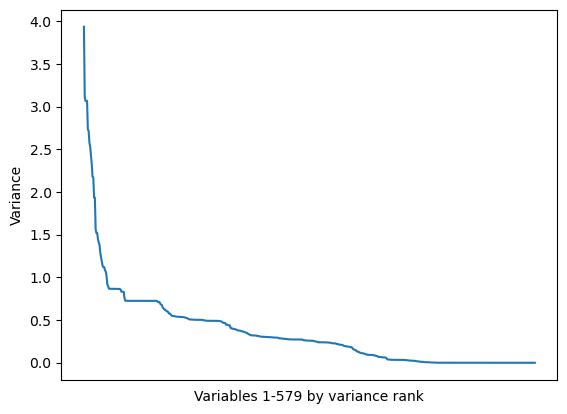
\includegraphics[width=\columnwidth]{Figures/Graphs/Total_variance}
\caption{Scaled variance of all the variables}
\label{variance}
\end{figure}

\subsection{Variable vs feature}
In time series learning, the terms variable and feature are often used interchangeably, which can cause confusion. 
Crucially, variables are a type of feature. 
%\include{Chapters/Chapter4} 
%\include{Chapters/Chapter5} 

%----------------------------------------------------------------------------------------
%	THESIS CONTENT - APPENDICES
%----------------------------------------------------------------------------------------

\appendix % Cue to tell LaTeX that the following "chapters" are Appendices

% Include the appendices of the thesis as separate files from the Appendices folder
% Uncomment the lines as you write the Appendices

% Appendix A

\chapter{Frequently Asked Questions} % Main appendix title

\label{AppendixA} % For referencing this appendix elsewhere, use \ref{AppendixA}

\section{How do I change the colors of links?}

The color of links can be changed to your liking using:

{\small\verb!\hypersetup{urlcolor=red}!}, or

{\small\verb!\hypersetup{citecolor=green}!}, or

{\small\verb!\hypersetup{allcolor=blue}!}.

\noindent If you want to completely hide the links, you can use:

{\small\verb!\hypersetup{allcolors=.}!}, or even better: 

{\small\verb!\hypersetup{hidelinks}!}.

\noindent If you want to have obvious links in the PDF but not the printed text, use:

{\small\verb!\hypersetup{colorlinks=false}!}.

%\include{Appendices/AppendixB}
%\include{Appendices/AppendixC}

%----------------------------------------------------------------------------------------
%	BIBLIOGRAPHY
%----------------------------------------------------------------------------------------

\printbibliography[heading=bibintoc]

%----------------------------------------------------------------------------------------

\end{document}  
